%%%%%%%%%%%%%%%%%%%%%%%%%%%%%%%%%%%%%%%%%%%%%%%%
% COPYRIGHT: (C) 2013-2015 FAU FabLab and others
% Bearbeitungen ab 2015-02-20 fallen unter CC-BY-SA 3.0
% Sobald alle Mitautoren zugestimmt haben, steht die komplette Datei unter CC-BY-SA 3.0. Bis dahin ist der Lizenzstatus aller alten Bestandteile ungeklärt.
%%%%%%%%%%%%%%%%%%%%%%%%%%%%%%%%%%%%%%%%%%%%%%%%


\newcommand{\basedir}{fablab-document}
\documentclass{\basedir/fablab-document}
% \usepackage{fancybox} %ovale Boxen für Knöpfe - nicht mehr benötigt
\usepackage{amssymb} % Symbole für Knöpfe
\usepackage{subfigure,caption}

\usepackage{marvosym} % für Briefumschlag-Symbol
\usepackage{eurosym}
\usepackage{tabularx} % Tabellen mit bestimmtem Breitenverhältnis der Spalten
\usepackage{wrapfig} % Textumlauf um Bilder
\renewcommand{\texteuro}{\euro}
\usetikzlibrary{shadings}

\usepackage[colorinlistoftodos,prependcaption]{todonotes}
\presetkeys%
{todonotes}%
{inline,backgroundcolor=red}{}

\linespread{1.2}

\date{Januar 2013}
\author{kontakt@fablab.fau.de}
\fancyfoot[L]{kontakt@fablab.fau.de}
\title{Einweisung Schneideplotter}

\tikzstyle{plotterknopf} = [anchor=base, draw=black, fill=gray!10, rectangle, rounded corners, inner sep=2pt, outer sep = 3pt]

% Knöpfe für Laser und Fernbedienung
\newcommand{\knopf}[2]{
    \begin{tikzpicture}[baseline={(box.base)}]
    \node [#1] (box) { 
        \fontsize{9pt}{9pt}\selectfont \textbf{#2}\strut
    };
    \end{tikzpicture}
}

\newcommand{\pfeil}{\ensuremath{\rightarrow}}

\newcommand{\plotterKnopf}[1]{\knopf{plotterknopf}{#1}}
\newcommand{\plotterDisplay}[1]{\texttt{#1}}

% einzelne Knöpfe
\newcommand{\plotterTest}{\plotterKnopf{TEST}}
\newcommand{\plotterOrigin}{\plotterKnopf{ORIGIN}}
\newcommand{\plotterPause}{\plotterKnopf{PAUSE}}
\newcommand{\plotterMenu}{\plotterKnopf{MENU}}
\newcommand{\plotterForce}{\plotterKnopf{FORCE}}
\newcommand{\plotterEnter}{\plotterKnopf{ENTER}}
\newcommand{\plotterPfeilRauf}{\plotterKnopf{$\blacktriangle$}}
\newcommand{\plotterPfeilRunter}{\plotterKnopf{$\blacktriangledown$}}
\newcommand{\plotterPfeilLinks}{\plotterKnopf{$\blacktriangleleft$}}
\newcommand{\plotterPfeilRechts}{\plotterKnopf{$\blacktriangleright$}}

\usepackage{siunitx} % SI-Einheiten ohne Gore

%\newcommand{\todo}[1]{\textbf{\color{red}{TODO: #1}}}


% Wenn wir die Zeichnungen aus der Anleitung nehmen, müssen wir entsprechend korrekt zitieren:
% in der Anleitung steht eigentlich, dass alle Auszüge etc verboten sind, aber Roland steht ja nicht über dem Urheberrecht
\newcommand{\RolandCopyrightHinweis}{Abbildung \copyright{} 2005 Roland DG Corporation, aus \texttt{\tiny http://files.rolanddg.be/Products/GX-24/Manuals/Manual\_GX-24\_de.pdf}}

\begin{document}
\maketitle
\section{Regeln und Hinweise}
\begin{itemize}
 \item Der Plotter ist empfindlich.
 \item Sei vorsichtig! Verstelle nichts, wenn du nicht ganz genau weißt, was du tust.
 \item Finger weg, wenn der Plotter arbeitet.
 \item Messerspitze nicht berühren, sie ist scharf und kann leicht beschädigt werden.
 \item Nur erlaubte Materialien (siehe Liste) mit dazu passendem Messer und ggf. Schneidunterlage verwenden.
\end{itemize}

\section{Erlaubte Materialien}
\paragraph{Dicke}
Es lassen sich Papiere und Folien bis zu einer Dicke von 0,1\,mm (Material ohne Trägerfolie) schneiden.
Die Gesamtdicke inklusive Trägerfolie darf bis zu 0,3\,mm betragen.

\paragraph{Größe}
Die Mindestmaße liegen bei 50\,mm Breite und 100\,mm Länge.
Höchstmaße 70\,cm breit (davon 63\,cm nutzbar), unendlich lang.

Bei einer Länge von über 50\,cm kann es vorkommen, dass die Folie während des Schneidevorgangs im Plotter verrutscht.
Wenn möglich, sollte das Motiv dann lieber in mehreren Einzelteilen ausgeplottet werden.
Wenn das nicht möglich ist, kann versucht werden die Folie möglichst gut aufliegen zu lassen (beispielsweise auf einem Tisch), so dass sie nicht herab hängt und stark zieht, und die Schnittgeschwindigkeit geringer zu stellen.


\paragraph{Materialien mit Trägerfolie}
Material mit einer Rückseite, die nicht durchgeschnitten wird:
\begin{itemize}
 \item PVC-Klebefolie für Beschriftungen
 \item Flex- und Flockfolie zum Bedrucken von Kleidung
 \item Selbstklebendes Etikettenpapier
\end{itemize}

\paragraph{Materialien ohne Trägerfolie}


Bei diesen Materialien (z.\,B. Overheadfolie oder normales Papier) muss eine Schneidunterlage verwendet werden,
entweder eine spezielle selbstklebende Schneideunterlage oder z.\,B. ein Stück Karton, das man mit Sprühkleber befestigt.  
\begin{itemize}
 \item Papier bis $$250 \frac{\mathrm{g}}{\mathrm{m}^2}$$, halte bei stärkerem Material Rücksprache (Achtung, 80g Papier reißt oft beim Ablösen von der Schneideunterlage!)
 \item Overheadfolie
 \item frage bei anderen Materialien bitte nach
\end{itemize}

\textbf{Ohne Unterlage wird die Schneidleiste des Plotters beschädigt!}
Zwei selbstklebende Unterlagen sind im FabLab vorrätig und befinden sich über dem Plotter in einer Kiste.
Das Material wird darauf gelegt und haftet an der Oberfläche des Trägers.
Dieser Stapel wird ganz normal in den Plotter eingeführt und eingespannt.
Nach dem Plotten ist darauf zu achten, dass sehr filigrane Strukturen beim Ablösen nicht zerstört werden.


\tableofcontents

\section{Das Gerät}
Bei dem Schneideplotter handelt es sich um ein Roland Camm-1 Servo GX-24. 

Mache dich kurz mit den Teilen des Plotters, welche du in der folgenden Zeichnung findest, vertraut.
Im weiteren Verlauf werden wir uns auf die entsprechenden Namen beziehen.

Die Knöpfe auf dem Bedienfeld werden folgendermaßen bezeichnet:
\plotterTest, \plotterOrigin, \plotterPause, \plotterPfeilRauf, \plotterPfeilLinks, \plotterPfeilRechts, \plotterPfeilRunter, \plotterMenu, \plotterForce und \plotterEnter.
Unten links findest du die Feinjustierung des Auflagedrucks, welcher auf 0 stehen sollte, sowie unten rechts den Netzschalter.
Im eingeschalteteten Zustand leuchtet der Netzschalter blau.
\begin{center}
 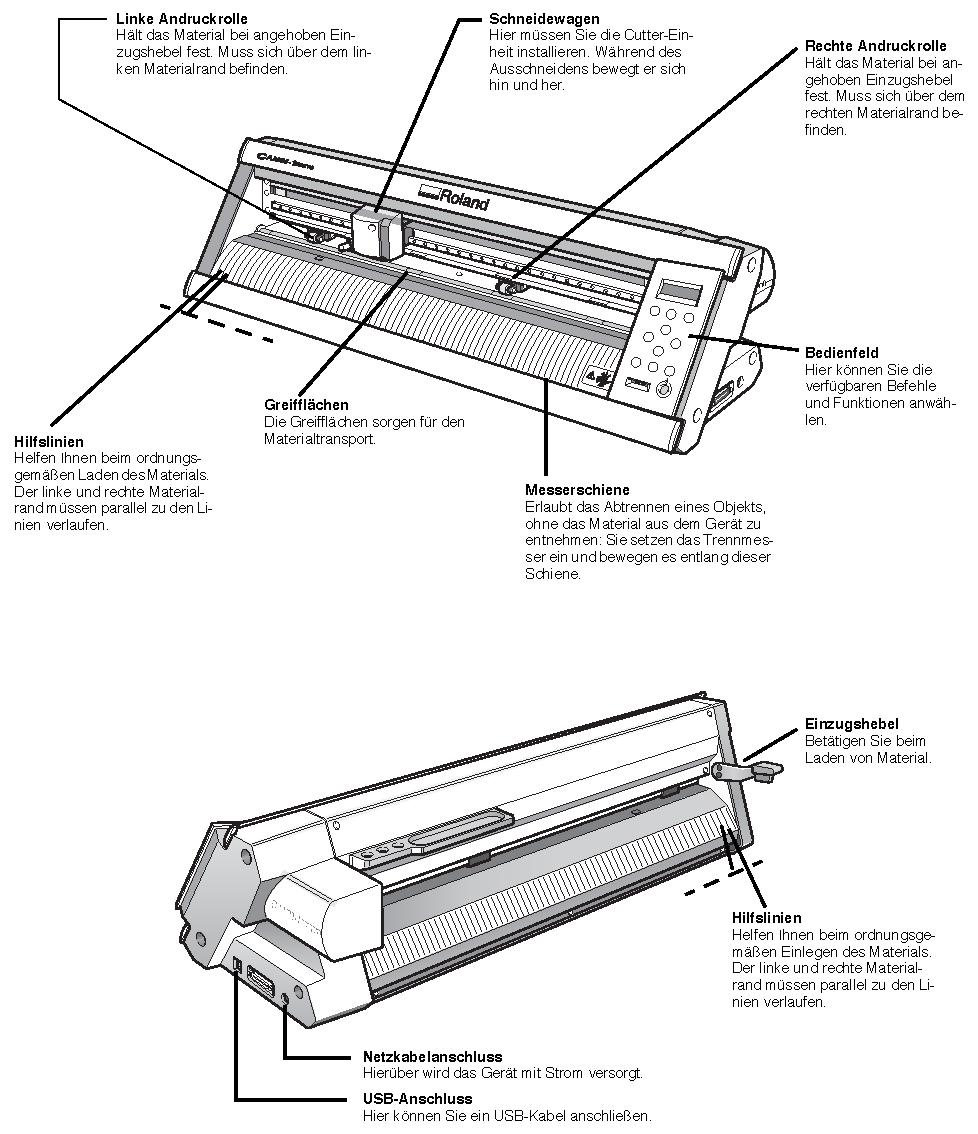
\includegraphics[width=\textwidth]{img/plotteroverview} \\
 \textbf{Aufbau des Plotters} \\
 \RolandCopyrightHinweis
\end{center}


\section{Anschalten und Material einlegen}
Als Erstes muss der Plotter angeschaltet werden.
Dazu den Netzschalter für eine Sekunden gedrückt halten, bis dieser blau leuchtet.

Danach den Einzugshebel (hinten links) absenken, um die Andruckrollen zu lösen.
Nun das Material von hinten einführen, bis es die Hilfslinien vorne erreicht.
Folie richtig herum einlegen, bei T-Shirt-Folie siehe Kapitel \ref{VerarbeitungShirtfolie}.

Durch Orientierung an den Hilfslinien kann man sicherstellen, dass das Material gerade eingelegt ist.
Wichtig ist, dass der rechte Materialrand genau unterhalb einer der grauen Kontrollmarkierungen liegt. \\
Siehe dazu folgende Zeichnung:
\begin{center}
 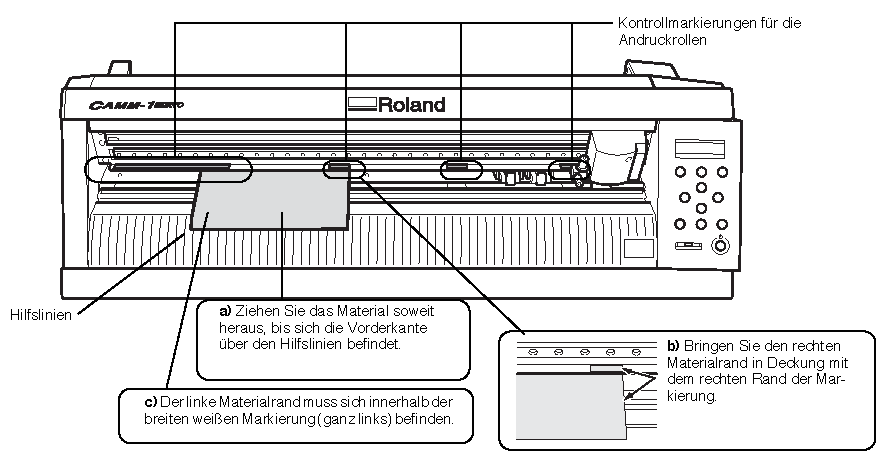
\includegraphics[width=\textwidth]{img/kontrollmarkierungen} \\
 \RolandCopyrightHinweis
\end{center}

Der linke Materialrand muss sich unterhalb der großen grauen Kontrollmarkierung befinden.
Dann müssen die Andruckrollen positioniert werden.
Dabei ist auch wieder darauf zu achten, dass sich  die linke Rolle innerhalb der großen Kontrollmarkierung befindet.
Die andere Andruckrolle muss in einem der vier grauen Bereiche liegen.
Positioniere die rechte Rolle so, dass der Abstand zwischen den Rollen möglichst groß ist.
Beide Rollen müssen sich aber vollständig auf dem Material befinden.  

\begin{center}
\begin{tabularx}{\textwidth}{X|XX}
        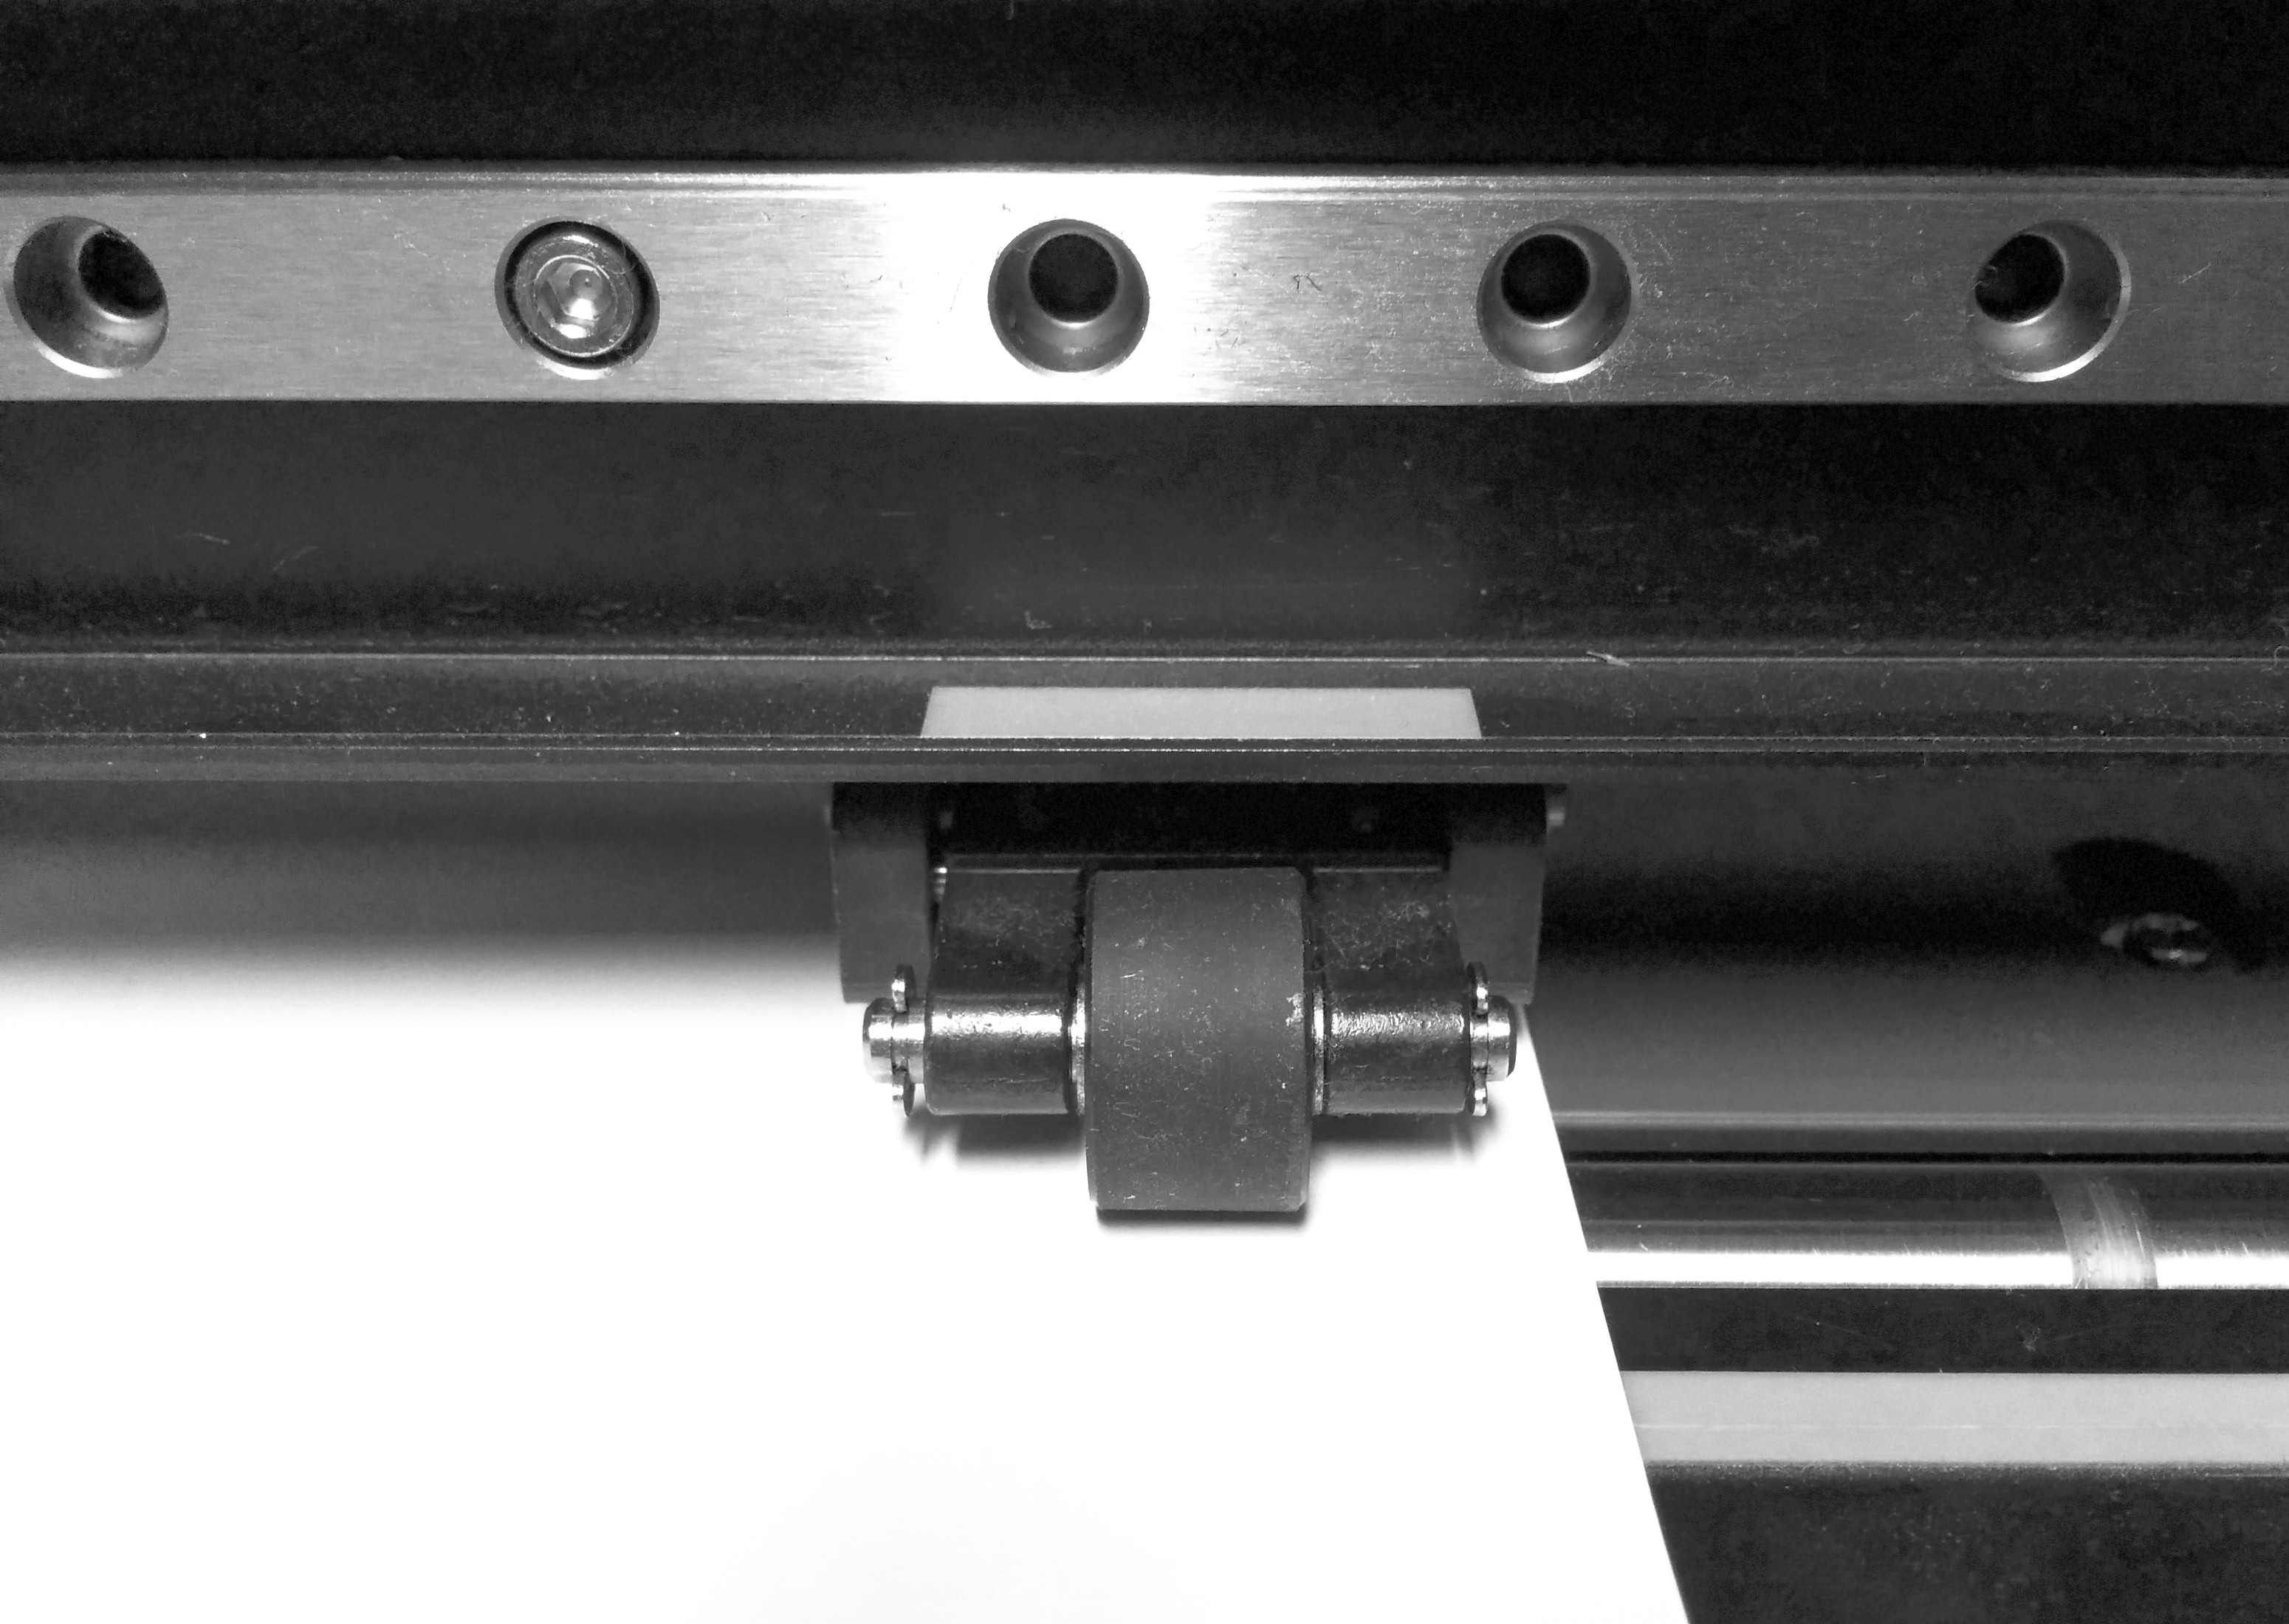
\includegraphics[width=0.3\textwidth]{img/correct.jpg}
    &
        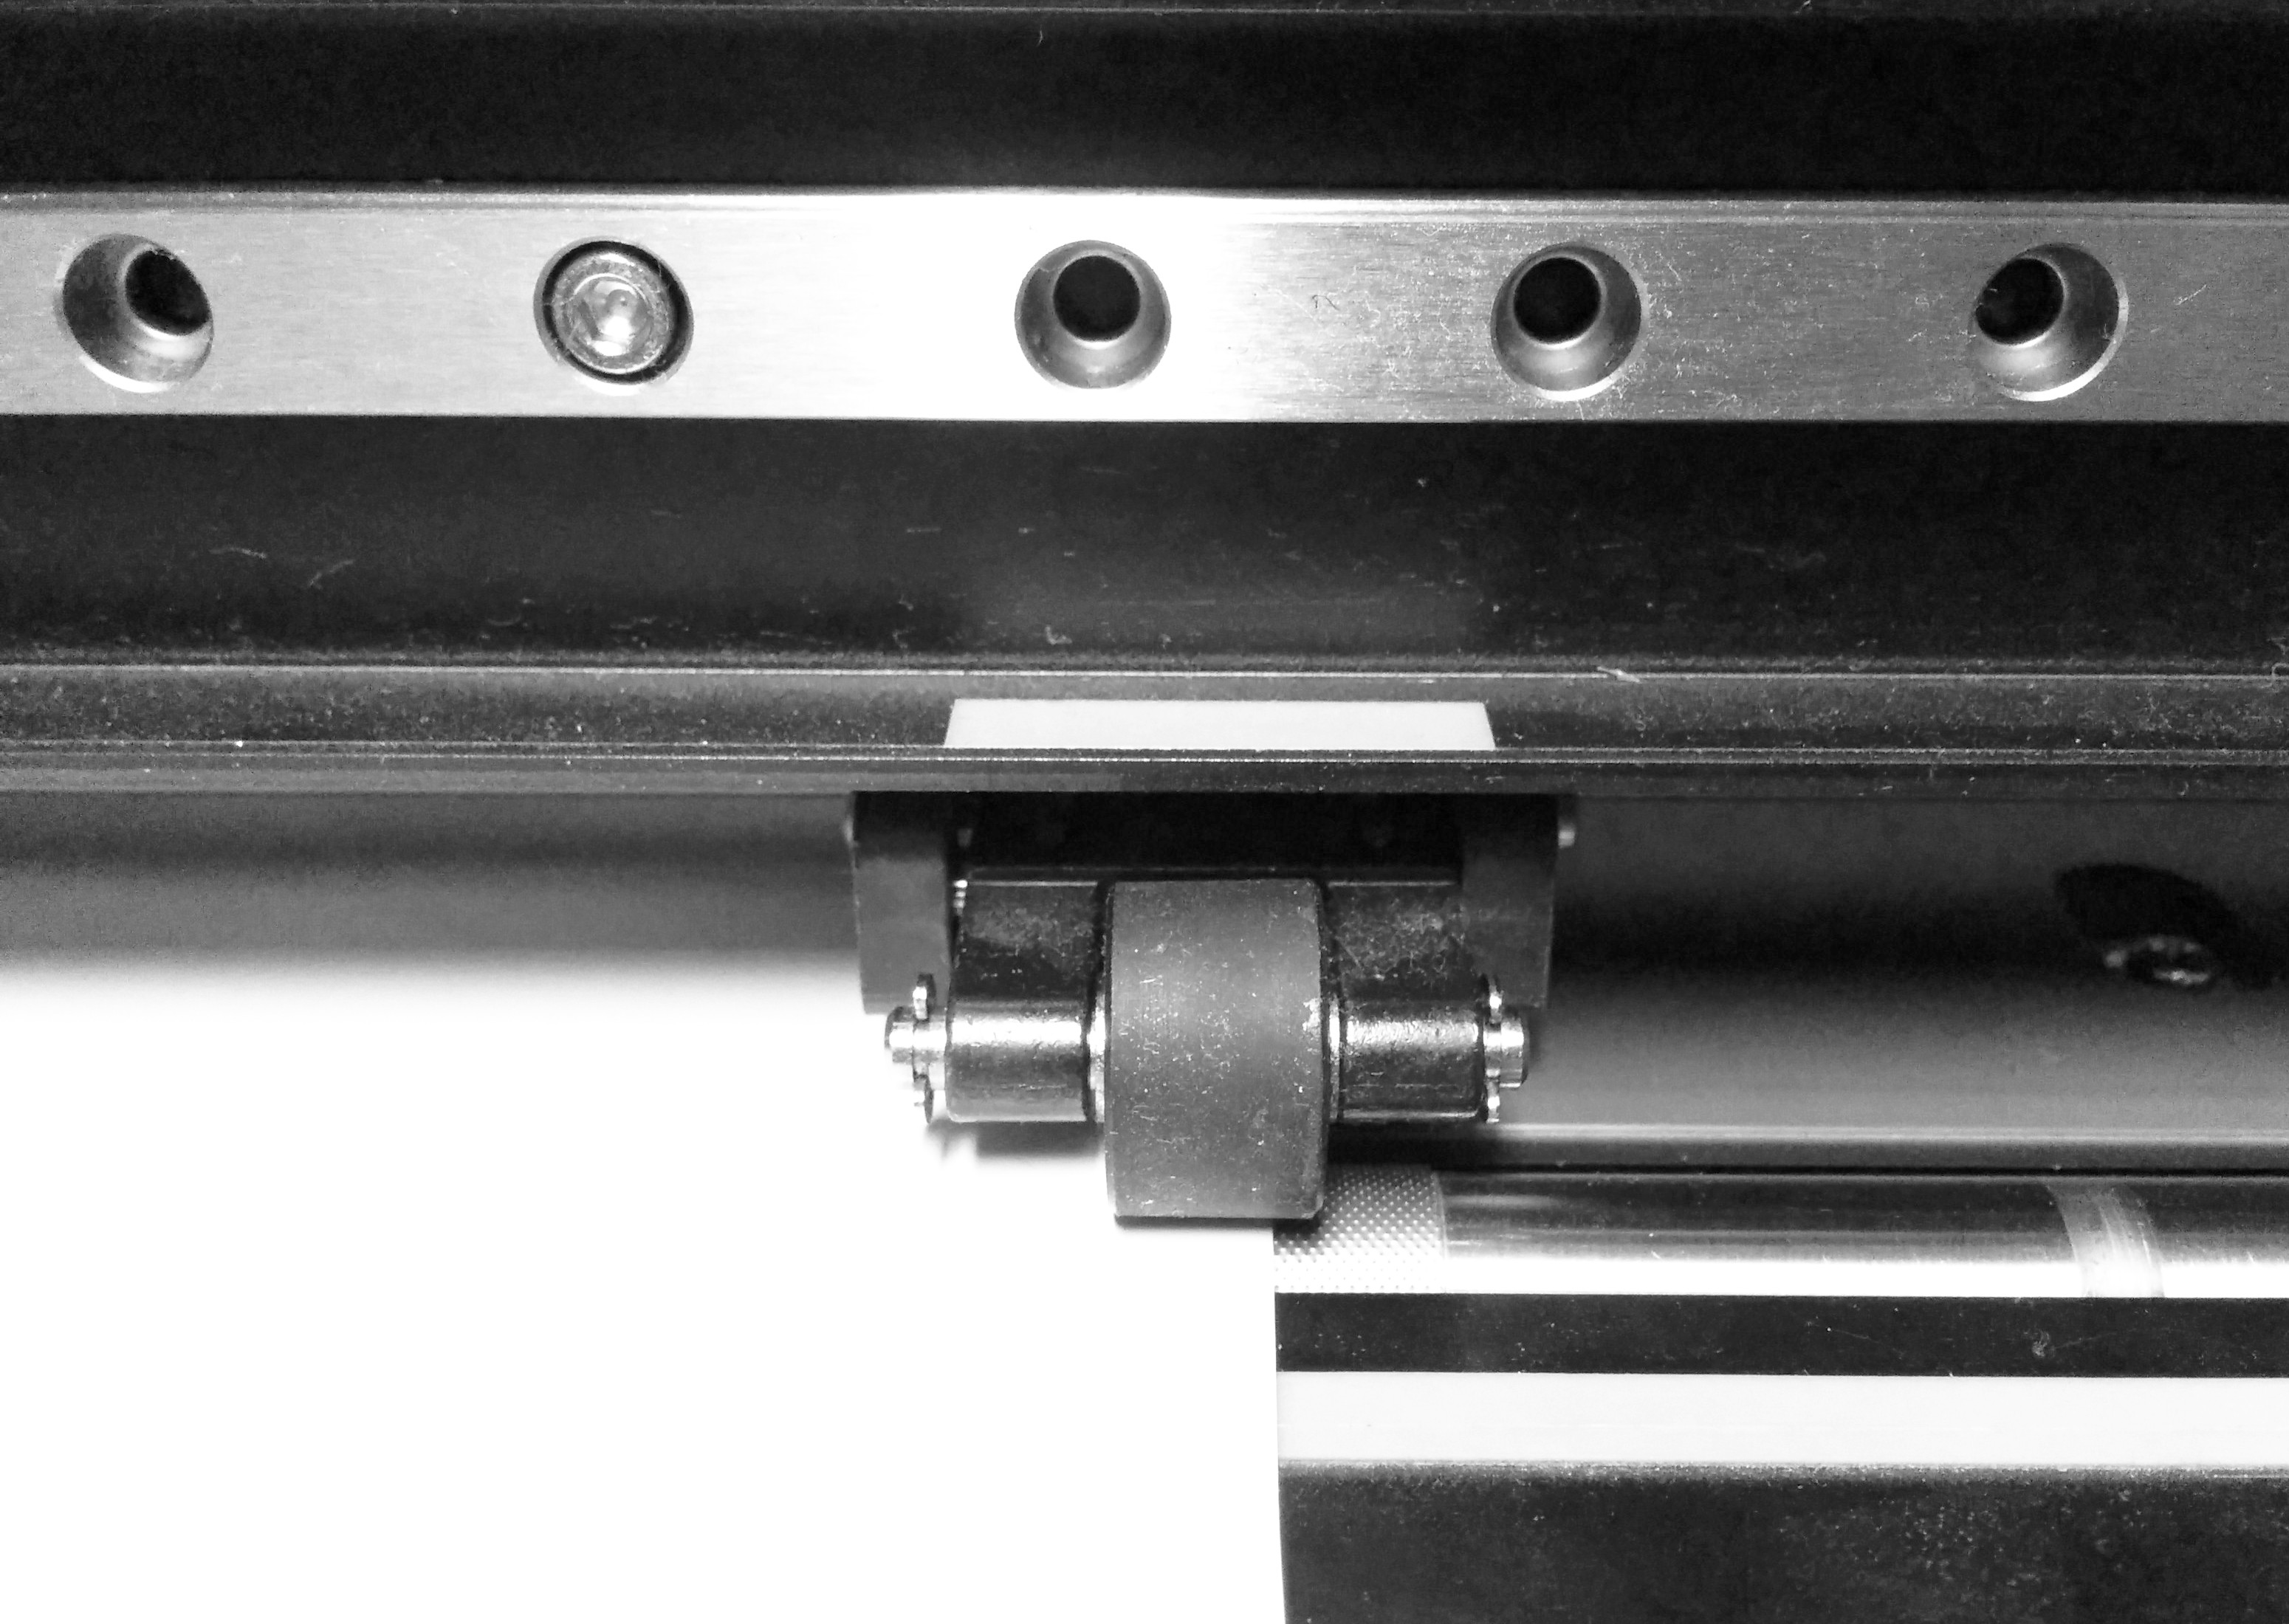
\includegraphics[width=0.3\textwidth]{img/wrong_foil.jpg}
    &
        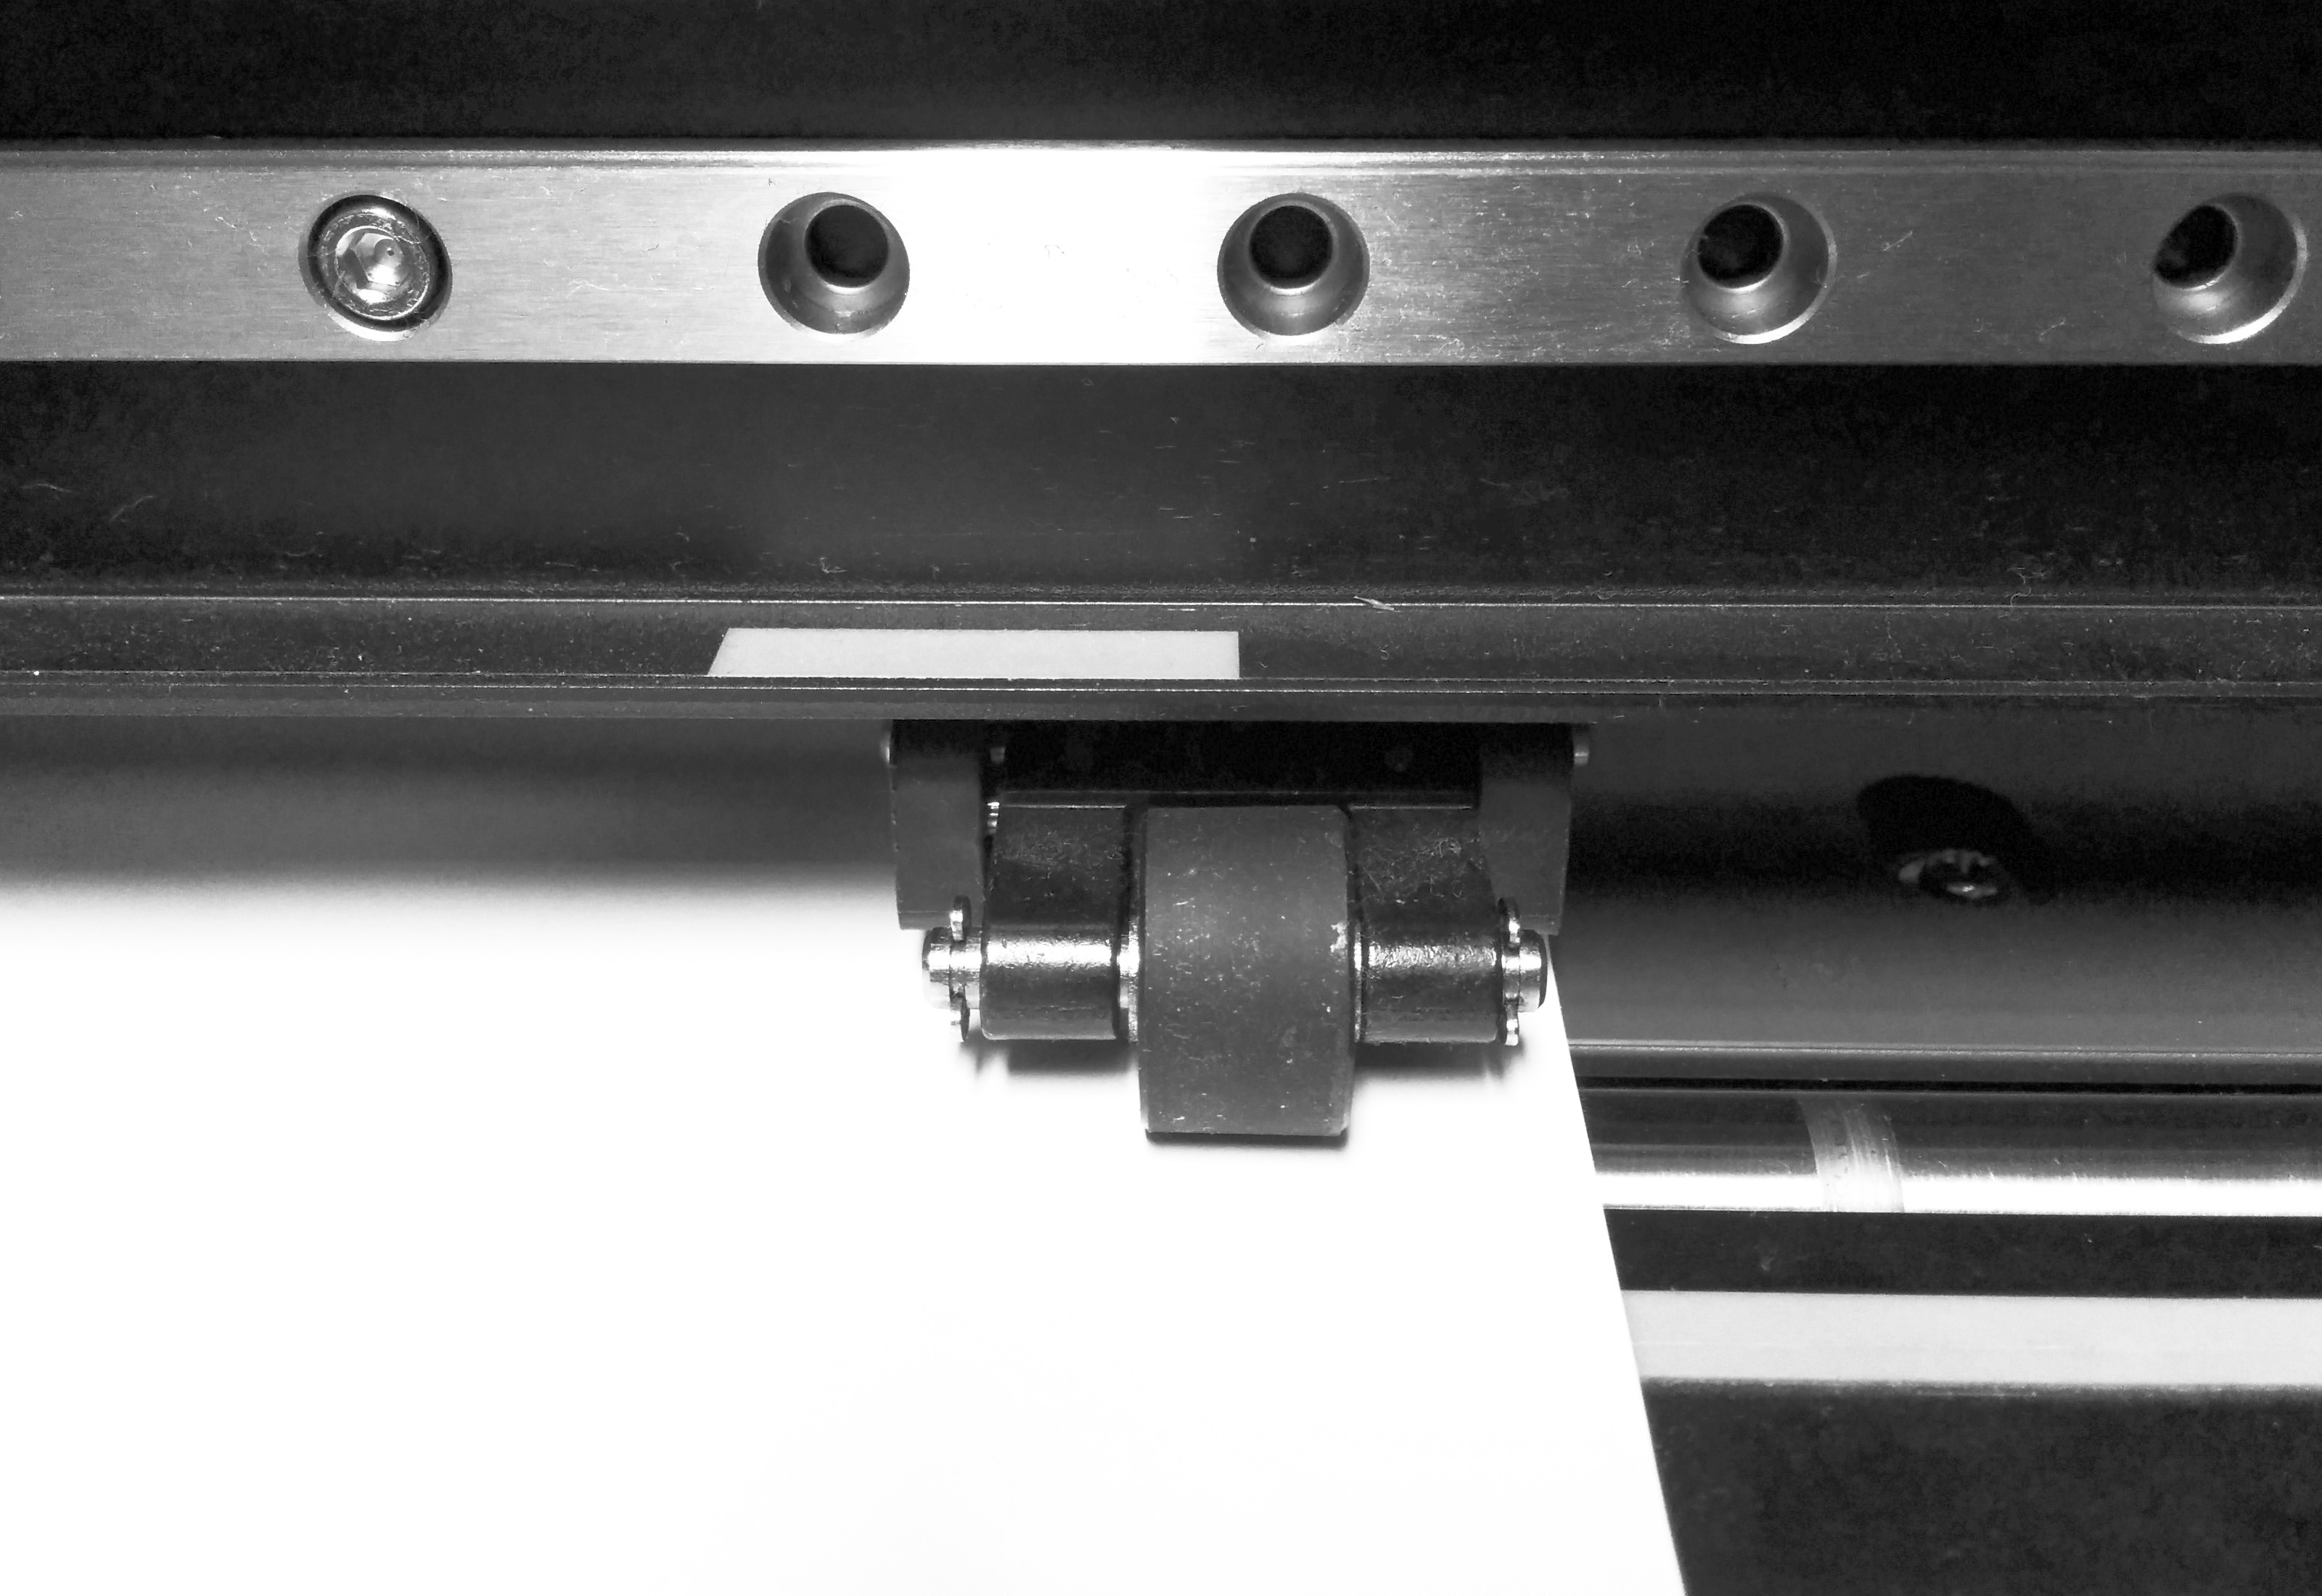
\includegraphics[width=0.3\textwidth]{img/wrong_role.jpg} \\
        \center \textbf{Richtig}
    &
        \center \textbf{Falsch:}\\ Die Rolle muss vollständig auf der Folie fahren.
    &
        \center \textbf{Falsch:}\\ Die Rolle muss sich innerhalb der markierten Bereiche befinden.
\end{tabularx}
\end{center}

Wenn das Material fertig eingelegt ist, musst du den Einzugshebel hochklappen, um das Material zu fixieren.

Auf dem Display solltest du folgendes sehen: \plotterDisplay{SELECT SHEET}.
Nun musst du dich entscheiden ob du aus einer Rolle etwas ausschneiden möchtest oder von einem Blatt (d.\,h. alles was kürzer als 1,6\,m ist).

\paragraph{Rolle (oder Kante)}
Wähle mit den Tasten \plotterPfeilRauf \plotterPfeilRunter entweder \plotterDisplay{KANTE} oder \plotterDisplay{ROLLE} aus und bestätige mit \plotterEnter die Auswahl.
Wenn du \plotterDisplay{ROLLE} auswählst, liegt der Nullpunkt für dieses Material auf der Schneidekante.
Das ist der hellblaue Gummistreifen unterhalb des Schneidewagens.
Wenn du aber \plotterDisplay{KANTE} auswählst, dann wird die Anfangskante der Rolle gesucht und 1,5-2\,cm bis zum Nullpunkt Platz gelassen.

\paragraph{Blatt}
Wenn Du stattdessen Blatt wählst, zieht der Plotter das eingelegte Blatt einmal vollständig ein, und schiebt es danach wieder zurück um die Maße zu bestimmen.
Diese werden danach im Display angezeigt.

Nach dem Einlegen und der Auswahl der Medienart musst Du auf jeden Fall so lange warten, bis die Medienmaße im Display angezeigt werden.
In den Modi Rolle und Kante wird für die Länge \enquote{---} angezeigt.

Danach einmal den Knopf \plotterMenu drücken um das Laden abzuschließen.


\section{Material einstellen (nach Tabelle)}

Je nach Material musst du nun die Einstellungen herausfinden:
\begin{itemize}
 \item Messertyp
 \item Schnitttiefenbegrenzung (am Messerhalter)
 \item Offset des Messers (Einstellung im Plotter)
 \item Geschwindigkeit und Schnittkraft (Einstellung im Plotter)
\end{itemize}

Dazu haben wir Tabellen zusammengestellt.
Wenn dein Material nicht enthalten ist oder die Einstellungen nicht funktionieren, lies in Abschnitt
\ref{einstellungenSelberAusprobieren} nach, wie du die Einstellungen selbst ermitteln kannst.

\subsection{Einstellungen und Messertyp ablesen}
\label{subsec:einstellungen}
In folgender Tabelle findest du zu gängigen Materialien das passende Messer und die Einstellungen.
Das Offset kannst du später anhand des Messertyps herausfinden.

\begin{tabular}{ccccc}
\hline
\textbf{Material} & \textbf{Andruck} & \textbf{Speed} & \textbf{Messer} & \textbf{Eintauchtiefe}\\
\hline
\hline
PVC Beschriftungsfolie & 100gf & 20cm/s & Rot & 0,15\,mm ? \\ \hline
Flockfolie & 100gf & 20cm/s & Grün & 0,3\,mm ** \\ \hline
Flexfolie & 100gf & 20cm/s & Rot & 0,15\,mm ? \\ \hline
250g Papier schneiden & 250gf & 20cm/s & Rot\\ \hline
250g Papier anreißen & 100gf & 20cm/s & Rot\\ \hline
Etikettenpapier schneiden & 70gf? & 20cm/s & Rot\\ \hline
Stiftplot Fineliner & 30gf & 30cm/s & Stift & --\\ \hline
Stiftplot Bleistift HB & 250gf & 20cm/s & Stift & --\\ \hline
\hline
\end{tabular}

{\footnotesize ** bei Flockfolie werden nicht die Fasern geschnitten, sondern nur die etwa 0,15\,mm starke Heißklebeschicht. Die Fasern hängen untereinander nicht zusammen.}

Das Offset zum jeweiligen Messer steht auf der Packung und als Richtwert auch hier in dieser Tabelle:

\begin{tabular}{ccccp{20em}}
\hline
\textbf{Kappen Farbe} & \textbf{Offset} & \textbf{Grad} & \textbf{max. Tiefe}* & \textbf{Geeignet für...}\\
\hline
\hline
Rot & 0,3\,mm & 45$^{\circ}$ & 0,3\,mm & normale Beschriftungsfolie (nicht Reflex/Glitzer!), Flexflolie, Papier, Overheadfolie\\
\hline
Rot small & TODO & 45$^{\circ}$ & TODO & wie Rot, für kleinste Schriften\\
\hline
Blau & 0,3\,mm & 35$^{\circ}$ & 0,2\,mm &  besonders dünne Folien (ähnlich wie 45$^{\circ}$)\\
\hline
Grün & 0,5\,mm & 60$^{\circ}$ & 0,8\,mm & Flockfolien, reflektierende Folien, Karton, Filz (?) % TODO Filz behauptet Plottermeisterei.de, noch zu testen (Dicke?)
 \hfill\, % Workaround für Zeilenumbruch
 \mbox{dickes/weiches/zähes Material} \\
\hline
Weiß& 0,3\,mm & k.A. & k.A. & \todo{ergoogeln}\\
\hline
Stifte & 0\, mm & -- & -- & Malen\\
\hline
\end{tabular}

{ \footnotesize * Dieser Wert ist eine theoretische Obergrenze, die Einstellung muss je nach Material kleiner gewählt werden! Theoretisch maximale Eintauchtiefe = Offset $\cdot$ tan($\alpha$), sonst wird das effektive Offset negativ. }

Bei der Messerauswahl ist zu beachten, dass ein größerer Schneidenwinkel für dickere Materialien und feine Ausschnitte besser geeignet ist, dafür aber schneller verschleißt.
\newcommand{\messer}{
\shadedraw[left color=black!80!white!90!blue,right color=black!30!white] (-0.7,3) -- (-0.7,0) -- (-.2,0) -- (-.2,-2) -- (.7,0) -- (.7,3) -- cycle;
\fill[fill,color=black!20!white] (-.2,-2) -- (.7,0)  -- (.7,.3) --  (-.2,-1.7) -- cycle;
\draw[thick] (-0.7,3) -- (-0.7,0) -- (-.2,0) -- (-.2,-2) -- (.7,0) -- (.7,3) -- cycle;
}
\newcommand{\messerhalter}{
\draw[ultra thick,fill=white!90!black,fill opacity=50] (-2,2.5) -- (-2,-1) .. controls (-2,-1.66) and (2,-1.66) .. (2,-1) -- (2,2.5) -- cycle;
\node at (-.8,2) {Messerhalter}; 

\draw[dashed] (0,-1.6) -- (0,1.8);
\draw[->,very thick] (2.2,1.2) -- ++(1,0) ;
}
\begin{center}
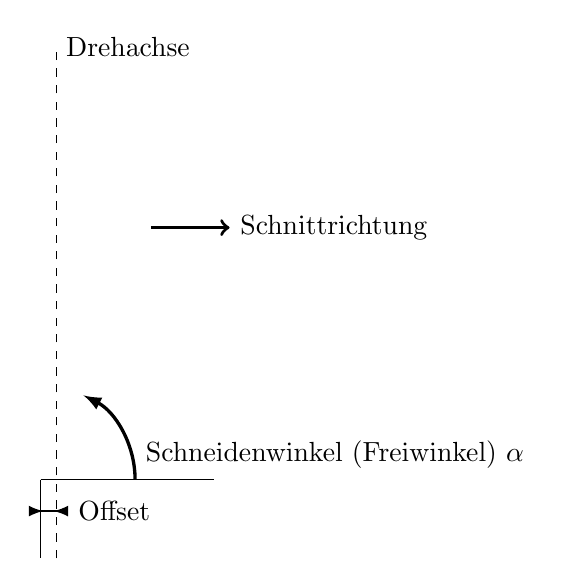
\begin{tikzpicture}
\messer 
\draw[dashed] (0,-3) -- (0,3.5) node[right] {Drehachse};
\draw (-0.2,-2) -- (2,-2);
\draw[-latex,very thick]  (1,-2) node[above right] {Schneidenwinkel (Freiwinkel) $\alpha$} arc (0:63:1.2)  ;
\draw (-.2,-2) -- (-.2,-3);
\draw[latex reversed-latex reversed,thick] (-.35,-2.4) -- (.15,-2.4) node[right] {Offset};
\draw[->,very thick] (1.2,1.2) -- ++(1,0) node[right] {Schnittrichtung};
\end{tikzpicture} 
\end{center}


\subsection{Messerwechsel und Tiefeneinstellung}

Wenn nicht das richtige Messer im Plotter geladen ist, musst du das Messer wechseln.
Auch für die Tiefeneinstellung muss der Messerhalter entnommen werden.

\label{messerwechsel}


\begin{enumerate}
 \item Zum Messerwechsel die silberne Halterungsschraube lösen und den Messerhalter entnehmen. \\
       Wenn das Messer nicht gewechselt werden soll, überspringe die nächsten vier Punkte.
 \item Oben auf den Stift drücken, damit das Messer unten herausschaut. 
 \item Dann, ohne sich zu stechen, das Messer herausziehen. 
\item Altes Messer mit Kappe versehen und aufräumen. Kappe des neuen Messers abziehen, ohne sich zu stechen.
\item Neues Messer in den Messerhalter tun. Kappe des neuen Messers aufräumen.\\ Am Plotter einen Notizzettel anbringen, welches Messer eingesetzt ist (Typ, Offset, Tiefeneinstellung).
\item Zur Einstellung der Tiefenbegrenzung zunächst den Messerhalter so drehen, dass die Messerspitze gerade im Messerhalter verschwindet. Wenn man jetzt den Messerhalter vorsichtig über ein Blatt Papier bewegt, soll er eine möglichst feine, aber gerade noch erkennbare Messerspur hinterlassen. Das entspricht einer Schnitttiefe von 0\,mm. 
\item Drehe nun den unteren Ring am Messerhalter, um die richige Eintauchtiefe einzustellen. Diese steht in der Material-Tabelle. \\Die auf dem Messerhalter angebrachten kleinen Striche entsprechen jeweils 0,05\,mm, eine ganze Umdrehung entspricht 0,5mm.

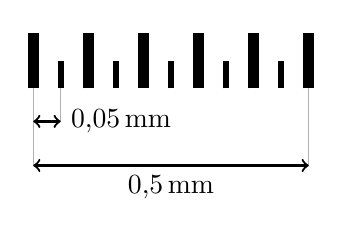
\begin{tikzpicture}[scale=0.7]
\draw[draw=black!30] (0,0) -- (0,-1.4);
\draw[draw=black!30] (0.5,0) -- ++(0,-.6);
\draw[draw=black!30] (5,0) -- ++(0,-1.4);
 \foreach \x in {0,1,2,3,4,5} {
    \draw[line width=4pt] (\x,0) -- ++(0,1);
 }
 \foreach \x in {0,1,2,3,4} {
    \draw[line width=2pt] (\x,0) ++(0.5,0) -- ++(0,0.5);
 }
\draw[<->,thick] (0,-1.4) -- ++(5,0) node[midway,below] {0,5\,mm};
\draw[<->,thick] (0,-.6) -- ++(.5,0) node[right] {0,05\,mm};

\end{tikzpicture}
\item Den Messerhalter wieder einsetzen, dabei die silberne Halterungsschraube mit der Hand leicht abstützen (gerade halten), da es sonst ungenau wird. Dann die silberne Halterungsschraube festziehen.
\end{enumerate}


\subsection{Offset}
Abschließend musst Du noch das Offset des eingesetzten Messers im Plotter einstellen.
Das Offset steht auf der Packung des Messers und auch in der Messer-Tabelle weiter oben.

Stelle es am Plotter mit \plotterMenu \pfeil \plotterDisplay{Kondition} \pfeil \plotterDisplay{Offset} ein.






\subsection{Anpressdruck}
Der Anpressdruck muss je nach Material eingestellt werden (siehe Tabelle weiter oben), dazu \plotterMenu so
oft drücken bis ungefähr folgendes angezeigt wird:\\
\plotterDisplay{20cm/s\\100gf 0.250mm}

Hierbei sind die \plotterDisplay{100gf} der eingestellte Anpressdruck, kontrolliere mit der gegebenen
Tabelle ob der eingestellte Anpressdruck zu deinem Material passt.

Mit \plotterForce \plotterPfeilRechts kann man den Anpressdruck ändern.
Mit \plotterPfeilRauf/\plotterPfeilRunter den Wert auswählen und dann \plotterEnter drücken.

\subsection{Geschwindigkeit}
Die Schnittgeschwindigkeit kann für die meisten Materialien bei \plotterDisplay{20cm/s} belassen werden.
Details können der Tabelle in Kapitel \ref{subsec:einstellungen} entnommen werden.
Ein Indiz dafür, dass die Schnittgeschwindigkeit zu hoch ist, ist dass das Messer spitze Ecken von der Trägerfolie abzieht.
\textbf{Achtung:} bei viel zu hoher Schnittgeschwindigkeit kann das Messer zerstört werden.


\todo{Wie stellt man Schnittgeschwindigkeit im Plotter ein und überprüft sie?}

\section{Einstellungen testen und selbst ermitteln}
\label{einstellungenSelberAusprobieren}
Normalerweise werden Anpressdruck und Tiefenbegrenzung einfach nach Tabelle eingestellt.
Wenn es damit funktioniert, kannst du diesen Punkt einfach überspringen.

\subsection{Testschnitt}
Falls du die Einstellungen testen möchtest, tue folgendes:
\begin{enumerate}
 \item Material einlegen wie weiter unten beschrieben
 \item an eine unwichtige Stelle fahren und \plotterTest gedrückt halten. Der Plotter schneidet nun rechts oben neben der aktuellen Messerposition einen Kreis mit einem innenliegenden Quadrat.
\item Ziehe nun den Kreis ab. Das Quadrat sollte nicht mit abgehen.
\item Ziehe das Quadrat ab. Du solltest unter dem Quadrat eine feine Messerspur erkennen können. Wenn sie zu tief ist, ist der Druck zu hoch. Wenn sie kaum erkennbar ist, ist der Druck zu niedrig. Wenn eine Erhöhung des Drucks nur wenig bringt, ist die Tiefenbegrenzung falsch eingestellt.
\end{enumerate}

\subsection{richtige Tiefenbegrenzung ermitteln}

Die Schnitttiefenbegrenzung ist dazu da, dass auch im Fehlerfall (doppelt geschnittene Linien oder zu hohe Kraft) das Messer nicht zu tief eintauchen kann.
Im richtigen Fall ist die Tiefenbegrenzung nur ein bisschen größer als die normale Eindringtiefe des Messers.

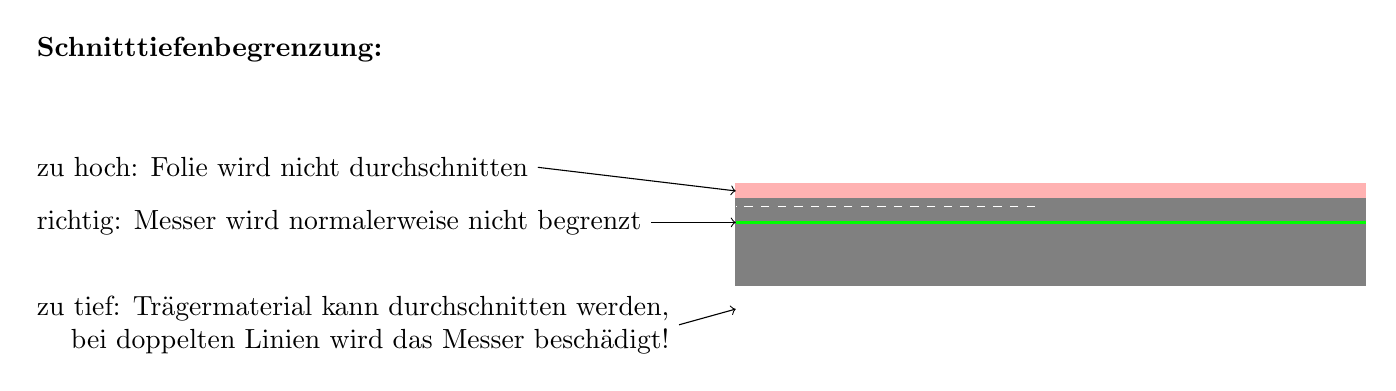
\begin{tikzpicture}
\tikzstyle{erklaerungstext}=[anchor=west, align=right];
\draw[fill,red!30!white] (-4,-1.9) rectangle (4,-1.7);
\draw[fill,black!50!white] (-4,-1.9) rectangle (4,-3);
\draw[draw=white,dashed] (-.2,-2) -- (-4,-2);
\draw[draw=green,very thick] (-4,-2.2) -- (4,-2.2);
\node[erklaerungstext] (zutief) at (-13,0) {\textbf{Schnitttiefenbegrenzung:}};
\node[erklaerungstext] (zutief) at (-13,-3.5) {zu tief: Trägermaterial kann durchschnitten werden,\\ bei doppelten Linien wird das Messer beschädigt!};
\node[erklaerungstext] (okay) at (-13,-2.2) {richtig: Messer wird normalerweise nicht begrenzt};
\node[erklaerungstext] (zuhoch) at (-13,-1.5) {zu hoch: Folie wird nicht durchschnitten};
\draw[->]  (zuhoch.east) to (-4,-1.8);
\draw[->]  (okay.east) to (-4,-2.2);
\draw[->]  (zutief.east) to (-4,-3.3);

\messer
\messerhalter
\end{tikzpicture}

Wenn trotz richtigem Anpressdruck die Folie nicht sauber durchgeschnitten wird, ist womöglich die Tiefenbegrenzung zu knapp eingestellt. 

Du musst jetzt selbst Schneideplotter spielen:
Hole dir zum Ausprobieren ein Teststück Folie und lege darunter einen Karton oder eine weiche Schneidunterlage.
Entnehme den Messerhalter, stelle die Tiefenbegrenzung auf 0 (Messer schaut nicht heraus) und fahre damit mit der Hand vorsichtig über die Folie.
Erhöhe die Tiefeneinstellung schrittweise um 0,05\,mm (ein kleiner Strich), bis die Folie gut durchschnitten wird.
Gib jetzt noch weitere 0,05\,mm als Reserve zu.

Als Faustformel für normale Klebe- und Flexfolien kann man \enquote{Materialstärke plus halbe Trägerdicke} nehmen.
Bei Flockfolie gilt das nicht!

Auf keinen Fall darf das Trägermaterial ganz durchschnitten werden, man darf auch keine Spuren auf der Rückseite sehen.
Bitte beachte die Maximaltiefe des Messers, die in der Messer-Tabelle steht.

\subsection{Anpressdruck ermitteln}

Sobald die Tiefenbegrenzung stimmt, kannst du den Anpressdruck so einstellen,
dass der Träger gerade leicht angeritzt wird.

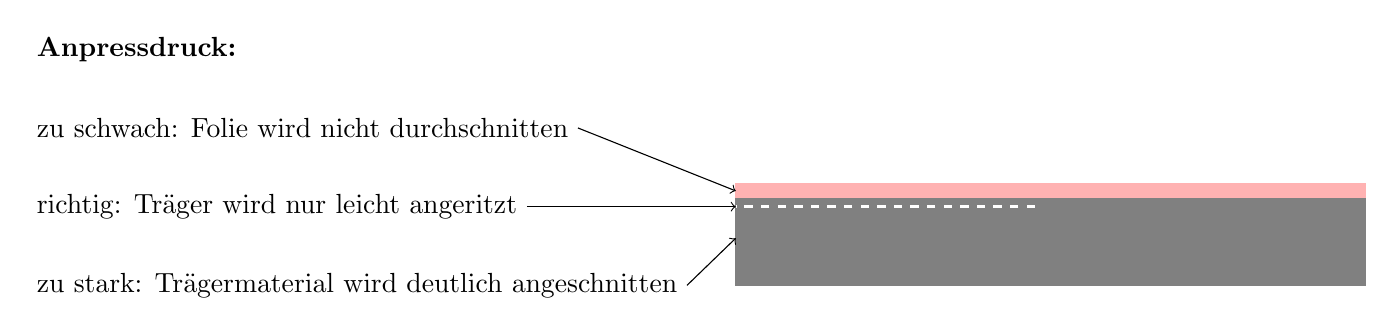
\begin{tikzpicture}
\tikzstyle{erklaerungstext}=[anchor=west];
\draw[fill,red!30!white] (-4,-1.9) rectangle (4,-1.7);
\draw[fill,black!50!white] (-4,-1.9) rectangle (4,-3);
\draw[draw=white,dashed,very thick] (-.2,-2) -- (-4,-2);
\node[erklaerungstext] (zutief) at (-13,0) {\textbf{Anpressdruck:}};
\node[erklaerungstext] (zutief) at (-13,-3) {zu stark: Trägermaterial wird deutlich angeschnitten};
\node[erklaerungstext] (okay) at (-13,-2) {richtig: Träger wird nur leicht angeritzt};
\node[erklaerungstext] (zuhoch) at (-13,-1) {zu schwach: Folie wird nicht durchschnitten};
\draw[->]  (zuhoch.east) to (-4,-1.8);
\draw[->]  (okay.east) to (-4,-2);
\draw[->]  (zutief.east) to (-4,-2.4);

\messer
\messerhalter
\end{tikzpicture}



\section{Nullpunkt festlegen}
Als Erstes legst du den Nullpunkt fest.
Wenn du das Material neu eingelegt hast, dann liegt der Nullpunkt dort, wo sich das Messer aktuell
befindet (linker Rand vom Material).
Das ist so auch richtig und muss normalerweise nicht weiter geändert werden.

Es kann nicht das komplette Material geschnitten werden, denn der Plotter hält 1,5-2\,cm Abstand zu allen Rändern.

Wenn du den Nullpunkt verändern möchtest, kannst du den Schneidewagen mit Hilfe der Pfeiltasten (\plotterPfeilLinks, \plotterPfeilRechts, \plotterPfeilRauf und \plotterPfeilRunter) verschieben.
Dabei siehst du auf dem Display, wieviel Platz zum rechten Rand, bzw. bis zur hinteren Kante verbleibt.
Um den aktuellen Punkt als Nullpunkt zu definieren, halte \plotterOrigin für zwei Sekunden gedrückt.

\section{Datei senden}
Die Datei muss eine Vektorgrafik (keine Pixel) sein.
Bei allen Objekten wird die Kontur geschnitten, auch verdeckte Konturen.
Das Motiv muss ggf. gespiegelt sein, bei T-Shirt-Folie siehe Kapitel \ref{VerarbeitungShirtfolie}.

\paragraph{Tipp:} Um später das Entgittern zu erleichtern, kann beim Erstellen der Datei auf runde Ecken geachtet werden.
Laufen zwei Konturen spitz aufeinander zu, so wird der Plotter an der Ecke absetzen und dadurch einen winzigen Steg lassen.
Wird der Pfad vorher verrundet, fährt der Plotter durch und schneidet so das ganze Material.

Öffne die Datei möglichst mit dem Programm, das sie erstellt hat. Starte von dort das CutStudio Plugin:

\begin{itemize}
 \item \textbf{Inkscape:} Datei öffnen, Erweiterungen\pfeil Roland CutStudio\pfeil Open. Dieses Plugin ist eine Eigenentwicklung, bitte melde alle Probleme mit der zugehörigen Datei an max@fablab.fau.de.

\item \textbf{Illustrator:} In der Menüleiste auf Fester $\rightarrow$ CutStudio PlugIn klicken. Es öffnet sich ein Unterfenster von Roland CutStudio mit einem großem \enquote{R} als Symbol. Auf das R draufklicken.

\item \textbf{Corel:} \todo{Plugin-Knopf in Corel}

\item \textbf{direkter Import:} Du kannst die Datei auch direkt in CutStudio importieren, starte dazu direkt CutStudio aus dem Startmenü. Der Import von CutStudio ist extrem wählerisch und funktioniert oft nicht.
\end{itemize}



In CutStudio auf Datei $\rightarrow$ Schneiden-Setup, Eigenschaften, Get from Machine, zweimal mit OK bestätigen.
Sollte eine Fehlermeldung \enquote{The machine is not responding} auftauchen, muss der Plotter aus- und eingeschaltet werden.
Wenn das auch noch nichts hilft, ausschalten und auf der rechten Seite den USB-Stecker, sowie das Netzkabel ziehen.
Jetzt den Eintaster betätigen um eventuelle Spannung im Gerät abzubauen.
Danach wieder alles einstecken und einschalten.

\textbf{Achtung:} Der Nullpunkt des Plotters befindet sich, wenn er nicht verschoben wurde, links unten auf der Folie.
Wenn deine Zeichnung nicht ebenfalls links unten auf der Seite beginnt, beginnt der Plotter nicht am Anfang der Folie, sondern verschwendet ein entsprechendes Stück!
Dieses muss dann i.\,d.\,R. auch bezahlt werden.

Im CutStudio auf Schneiden klicken und die Folie wird ausgeschnitten (Plotter fängt sofort an zu arbeiten!).
Sobald es fertig ist, mit \plotterPfeilRunter die Fole soweit ausfahen, bis das gesamte Motiv unterhalb der Schneidkante (Übergang zwischen grauem und schwarzem Kunststoff) ist.
An dieser Kante kann dann ein Messer angesetzt werden, um die Fole abzutrennen.
Die Rolle danach mit \plotterPfeilRauf nach hinten ausfahren, mit dem Hebel die Anpressrollen lösen und die Rolle hinten entnehmen.

Nun kannst du den Auftrag abschicken.

\section{Entgittern}
Nach dem Schneiden legst Du das geschnittene Material mit der Schutzfolie nach unten auf eine flache Oberfläche, und entfernst die Teile, die nicht zum fertigen Motiv gehören.
Dazu eignet sich ein schmaler, aber nicht zu spitzer Gegenstand, damit Du die Schutzfolie nicht aus versehen durchstößt, zum Beispiel ein Druckbleistift.
Es sind auch zwei Spezialwerkzeuge vorrätig, die du mit entsprechender Vorsicht verwenden kannst: Ein Haken (wie vom Zahnarzt) und ein Stift mit Messerspitze.

\section{Verarbeitung: Aufkleber}
Mit PVC-Folie kann man Aufkleber erstellen.
Dafür gibt es die Trocken- und die Nassmethode.
Die Vorbereitung ist für beide Methoden gleich.
\subsection{Ausschneiden}
Das Ausschneiden ist am Anfang dieser Einleitung beschrieben.
Folge den Anweisungen, bis du fertig entgittert hast.
Das Motiv muss seitenrichtig (nicht gespiegelt) ausgeschnitten werden, die Trägerfolie muss unten liegen. 

\subsection{Application Tape anbringen}
Nachdem du das Motiv geschnitten und entgittert hast, schneidest Du ein Stück Application Tape (Transferfolie) so aus, dass es das gesamtes Motiv abdeckt, und legst es über das Motiv.
Dabei kommt die Klebeseite des Application Tapes auf die Sichtseite des geschnittenen Motivs, so dass Du zum Schluss ein Sandwich mit den Schichten (von unten nach oben) \textit{Schutzfolie} - \textit{Geschnittenes Material} - \textit{Application Tape} hast.
Das Application Tape wird mit einer Rakel blasenfrei angedrückt, eventuelle Blasen mit einer Nadel vorsichtig aufstechen und glattstreichen.
Danach nochmals kräftig andrücken.
Du kannst danach das Trägermaterial und das Application Tape mit einem Messer zurechtschneiden.

\subsection{Anbringen eines Aufklebers - Vorbereitung}
Hilfsmittel:
\textbullet Fensterreiniger
\textbullet Spiritus
\textbullet Saubere fusselfreie Tücher
\textbullet Kreppband
\textbullet Rakel (Hilfsweise: Eiskratzer mit glatter Kante)
\textbullet Nadel (Zum Aufstechen von Blasen)
\textbullet Wasserwaage und/oder Metermaß

Der Untergrund auf dem der Aufkleber angebracht werden soll muss sauber und fettfrei sein.
Ab besten mit Fensterputzmittel abwaschen, trocknen, und dann (sofern es der Untergrund verträgt) nochmal mit Spiritus drüberreiben und gut trocknen lassen.

\subsection{Anbringen eines Aufklebers - Trockenmethode}
Bei der Trockenmethode haftet der Aufkleber sofort nach dem Anbringen auf den Untergrund.
Du musst daher die Ausrichtung bestimmen, bevor Du die untere Folie abziehst.

\subsubsection{Ausrichten}
Bei kleineren Aufklebern kann man das mit Augenmaß oder einer vorher auf dem Untergrund angebrachten Hilfslinie machen, dann die Trägerfolie (die untere Folie) abziehen, und den Aufkleber positionieren. 

Bei größeren Aufklebern empfiehlt es sich, erst den Aufkleber mit der Trägerfolie und dem Application Tape auf dem Untergrund auszurichten, und dann mit Kreppband am Application Tape zu fixieren, um Verrutschen zu vermeiden.

Bitte beachte, dass das Arbeiten mit einer Wasserwaage nur Funktioniert, wenn Du sicher sein kannst, dass das Objekt auf dem Du den Aufkleber anbringst selbst auch wirklich waagerecht steht.
Dies ist bei Autos zum Beispiel nicht sichergestellt.
Besser ist es, mit einem Maßband relativ zu einer Kante am Objekt auszurichten.

\subsubsection{Trägermaterial abziehen}
Danach ziehst Du von einer Seite ein Stück des Trägermaterials im \SI{180}{\degree}-Winkel ab, und bringst diesen Teil des Aufklebers durch Anrubbeln an.
Das Application Tape wird noch nicht entfernt.
Du kannst jetzt langsam weitere Teile des Trägermatierals abziehen (\SI{180}{\degree}-Winkel!) und anrubbeln,
bis Du schließlich das gesamte Trägermaterial entfernt hast.

Jetzt rubbelst Du den gesamten Aufkleber noch einmal sorgfältig mit der Rakel an.
Achte besonders darauf, dass Ecken und Kanten gut haften.
Falls Luftblasen sichtbar sind, versuchst Du diese vorsichtig auf kürzestem Weg zur Seite des Aufklebers zu drücken.
Falls das nicht möglich ist, stichst Du sie durch das Application Tape hindurch mit einer Nadel auf und rubbelst sie dann glatt.

\subsubsection{Application Tape abziehen}
Abschließend wird das Application Tape vorsichtig im \SI{180}{\degree}-Winkel abgezogen, und danach der gesamte Aufkleber noch ein letzes mal mit der Rakel angedrückt.

\subsection{Anbringen eines Aufklebers - Nassmethode}
Bei Nassmethode funktioniert nur auf glatten wasserundurchlässigen Untergründen.
Sie erlaubt dir, die Positionierung des Aufklebers nach dem Anbringen noch zu justieren. Dafür dauert das Trocknen nach dem Anbringen mehrere Stunden.

Nach der Reinigung des Untergrundes bringst Du dazu aus einer Sprühflasche eine feine Schicht destilliertes Wasser auf dein Untergrund auf.
Du kannst danach das Trägermaterial abziehen (\SI{180}{\degree}-Winkel!) und den Aufkleber samt Application Tape auf dem Untergrund aufbringen.
Er lässt sich in diesem Stadium noch verschieben und positionieren.  

Danach drückst Du den Aufkleber einmal vorsichtig mit der Rakel an, ohne ihn zu verschieben, prüfst auf Luftblasen (und drückst diese zur Seite aus dem Aufkleber) und lässt danach den Aufkleber samt dem Application Tape trocknen.
Wie lange das dauert, kann nicht pauschal gesagt werden, es hängt stark von der Luftfeuchte und den Temperaturen der Luft und des Untergrundes ab.
Rechne aber mit mehreren Stunden.

Nachdem der Aufkleber getrocknet ist, drückst Du ihn mit der Rakel gründlich an, und kannst danach das Application Tape im \SI{180}{\degree}-Winkel abziehen.
Abschließend drückst Du den Aufkleber noch ein letztes mal an. 

\section{Verarbeitung: Shirt-Folie} \label{VerarbeitungShirtfolie}
\subsection{Besonderheiten}
Die Shirtfolie besteht aus zwei Schichten: einem durchsichtigen Trägermaterial, das ganz am Ende entfernt wird, und einer farbigen, mit Schmelzkleber beschichteten PU-Folie.
Nur die bunte Folie wird geschnitten.

\begin{itemize}
 \item Bunte Seite nach oben einlegen! Oft ist dies die \emph{weniger} glänzende Seite. Da die Trägerfolie durchsichtig ist, kann man es nicht so einfach erkennen.
 \item Motiv muss \emph{gespiegelt} ausgeschnitten werden. (Da in die Rückseite des Materials geschnitten wird.)
 \item Nur die Länge kostet Geld, d.\,h. das Motiv auf Querformat drehen. Die Folie hat keine bevorzugte Verarbeitungsrichtung, d.\,h. längs oder quer ist egal.
 \item Folgende Farben der Flexfolie sind schwieriger zu verarbeiten und deshalb nur für größere Schriften (laut Hersteller ab 2\,cm) geeignet: hellblau, sämtliche Neonfarben und nachleuchtende Folie
 \item Ein bisschen Rand ist zur Verarbeitung nötig. Auf der linken Seite lässt der Plotter bereits selbst genug Rand, da man den Nullpunkt nicht ganz auf die Kante setzen kann.
\end{itemize}

\subsection{Motiv ausschneiden}
Das Motiv muss \textbf{gespiegelt} werden (Schrift spiegelbildlich).

Das weitere Vorgehen ist gleich dem Schneideplotten von anderen Materialien.
All dies ist am Anfang dieser Einweisung beschrieben und wird deshalb hier nicht wiederholt.
Bitte darauf achten, dass Andruckkraft und Messertyp richtig gewählt sind.

Für Flexfolien werden normale, rote Messer benötigt.
Andruckkraft ist moderat zu wählen.
Die Schnitttiefe ist so anzupassen, dass der Träger nicht durchtrennt wird.

Für Flockfolien muss das Messer getauscht werden.
Die richtige Messersorte und Tauschprozedur ist auf einem Aushang beim Schneideplotter beschrieben.

\subsection{Pressen}
Nachdem du das Motiv geschnitten und entgittert hast, muss es auf das T-Shirt übertragen werden.

Die T-Shirt-Presse einschalten, die Regelung ist auf den richtigen Temperatur- und Zeitwert einzustellen.
Die entsprechenden Werte werden entweder durch den Hersteller veröffentlicht oder sind auf der Heißpresse notiert.
Achtung: Das Oberteil der Presse wird jetzt heiß.
Nicht mehr berühren und Umstehende darauf hinweisen.
Das T-Shirt sollte am Besten aus Baumwolle sein, da auf Synthetikfasern die Haftung schlechter ist.

Das T-Shirt wird jetzt gerade und mittig eingelegt.
Dann die Folie richtigherum darauflegen: Schrift lesbar, buntes Material am T-Shirt, obendrüber das klare Trägermaterial.
Folie ausrichten (mittig zum T-Shirt? richtige Höhe?) und die weiße Antihaftmatte darauflegen.

Warten bis die Temperatur erreicht ist und die Presse mit viel Kraft schließen, bis sie einrastet.
Nach Ertönen des Signals die Presse rasch öffnen.
Nun die Trägerfolie abziehen, solange sie noch warm ist (bei normaler Flex- und Flockfolie).
Ausnahme: Bei Flexfolie in hellblau und Neonfarben die Folie erst im lauwarmen bis kalten Zustand abziehen.

Nachdem die Trägerfolie entfernt ist, nochmal das T-Shirt in die Presse einlegen.
Antihaftmatte auflegen und die Presse für 2 Sekunden schließen.
Wenn jetzt zu lange gepresst wird, bleibt die Matte auf dem T-Shirt kleben oder die Folie \enquote{verläuft}.

\subsection{Benutzungshinweise}
\todo{Bezahlung zu einem Kapitel für alle Folientypen machen und hier nur drauf verweisen.}
Dein T-Shirt ist jetzt fertig.
Bitte das Bezahlen nicht vergessen.
Die Preise der T-Shirtfolien sind auf Etiketten in den Rollen vermerkt.
Darin enthalten ist die Maschinennutzungsgebühr des Schneideplotters.
(Die Höhe dieser Gebühr ist auf einem Etikett am Plotter vermerkt.)
Wenn du eine Folie selbst mitbringst, musst du nur diese Nutzungsgebühr zahlen.
Für Folien aus der Restekiste entfällt diese Gebühr, da sie bereits gezahlt wurde.

Zusätzlich ist für die Benutzung der Presse ein Beitrag von 1€ zu zahlen.

\section{Verarbeitung: Glitzersteine applizieren}
\todo{testen und vollständig beschreiben}
Mit Hilfe des Plotters ist es möglich aus dicker Folie eine Schablone mit runden Löchern zu schneiden.
Diese wird auf Acryl aufgeklebt und in eine Kiste gelegt.
Mit einer Bürste können Heißkleber-beschichtete Glitzersteine in das Motiv eingebürstet werden.
Zum Übertrag wird die alte Transferfolie eine T-Shirt-Drucks genutzt.
Nun können die Steine auf ein T-Shirt heiß aufgetragen werden.
\section{Verarbeitung: Siebdruck}
\todo{testen und vollständig beschreiben}
Normalerweise sind zum Siebdruck beschichtete Siebe nötig.
Diese werden photochemisch entwickelt.
Da die zugehörige Chemie umfangreich und aufwändig in der Entsorgung ist, gibt es diesen Prozess nicht im FabLab.

Eine Alternative ist dicke Vinylfolie mit starkem Kleber und ein unbedrucktes Sieb zu kaufen.
Die Folie wird geschnitten und auf das Sieb oben drauf geklebt.
Nun kann das Sieb ganz normal zum Siebdruck verwendet werden.
\section{Verarbeitung: Zeichnungen plotten}
\todo{testen und vollständig beschreiben}
Mit dem Plotter ist prinzipiell auch Zeichnen möglich.
Dazu muss statt dem Messer ein Stift eingesetzt werden.
Grundsätzlich gilt beim Wechsel des Stiftes/Messers, den Messerhalter vorsichtig zu behandeln und gut aufzustützen.

Der Messerwechsel ist in Kapitel \ref{messerwechsel} beschrieben.
Prinzipiell wird einfach statt dem Messer ein Stifthalter eingesetzt.
Dieser lagert in der Werkzeughalterung an der Rückkante des Plotters.

Der Anpressdruck ist grunsätzlich so einzustellen, dass der Stift gerade noch ohne Aussetzer zeichnet.
Bei verschlisseneren Stiftspitzen, kann der Anpressdruck erhöht werden.
Wenn Schmierer und Nebenstriche entstehen, ist der Stift endgültig verschlissen.

\todo{wie hoch soll der Stift normal über dem Papier schweben? Wenn man es falsch macht, klappert es fürchterlich}

Ein interessantes Programm zur Pfaderzeugung aus Bildern gibt es hier: \url{http://www.evilmadscientist.com/2012/stipplegen2/}

Strich-Schriftarten: \url{http://www.evilmadscientist.com/2011/hershey-text-an-inkscape-extension-for-engraving-fonts/}

Schraffieren geht in Inkscape mit dem Pfad-Effekt Schraffur, der aber nicht auf Gruppen, sondern nur direkt auf Pfade angewendet werden muss.

\listoftodos

\newpage
\appendix
\section{Copyright}
Der Quelltext dieser Einweisung, ohne die Bilder von Roland, ist unter CC-BY-SA 3.0 Unported lizenziert. Solange kein freier Ersatz für die Roland-Bilder vorliegt, kann das gesamte Dokument leider nicht frei verwendet werden.
%\ccLicense{schneideplotter-einweisung}{Einweisung Schneideplotter}
\todo{freien Ersatz für die Bilder finden}

Dieses Dokument stammt aus fau-fablab/schneideplotter-einweisung@\Revision{}.

\end{document}
